\documentclass[../MasterThesis.tex]{subfiles}
\graphicspath{ {./assets/images/} }


%----------------------------------------------------------------------------
%----------------------------------------------------------------------------

\begin{document}
	
	
%
%
%
%
%=======================================================================================================
%
%
%
%
%=======================================================================================================
% CHAPTER: CONCLUSION AND FUTURE WORK
%=======================================================================================================
\newpage
\section{Conclusion} \label{section:conclusion}

In this Chapter, a summary of this thesis project, its contributions as well as its limitations are described. Afterwards, opportunities for future work are introduced and examined.






%-------------------------------------------------------------------------------------------------------
\subsection{Summary} \label{subsection:summary}
% Summarize the key findings and outcomes of the research.


The topic of this thesis project is on multimedia processing in real-time, regarding the adjustment of the RGB values of a video with JIT using the MLT framework as a backend. This solution was implemented in Codemill's Accurate Player and using WebRTC as a data channel.

In this thesis, background knowledge on colour theory and representation (Chapter~\ref{section:theoreticalfoundationofcolour}) and the technical background, especially the structure and usage of the MLT framework were given. Additionally protocol buffers and other streaming components were introduced in Chapter~\ref{section:technicalbackground}.

This thesis project explored two research questions. The first question aimed to evaluate the feasibility of the real-time colour grading with JIT and the MLT framework. The implementation as described in Chapter~\ref{section:designandimplementation} confirms that it was achievable. To select the most suitable MLT filter for the RGB adjustment, a comparison of different MLT filters was conducted. The selected filter is the \texttt{avfilter.colorbalance} filter, which can be used to adjust the RGB values of the highlights, midtones and shadows of a video individually and achieves the most vibrant and saturated results.


The second research question considers the comparison of video colour grading results with MLT filters that were applied on different platforms. The compared platforms are the Accurate Player that was implemented in this thesis project, the Melt CLI tool and KDEN Live (Chapter~\ref{section:experimentalevaluationanddiscussion}).
%
%
%To evaluate the differences, frames of the different platforms were extracted and compared. 
%The colours of those frames have been subtracted from each other using the \textit{grain extract} function in GIMP, to show differences in the colour saturations.
The comparison with Melt revealed an interesting result: The extracted frames display significant differences, even without the application of filters. This showed that the Accurate Player is presenting the original videos files more accurately than Melt does.
% The cause for those differences remains unclear.
The comparison with KDEN Live did not show the same results as the filter application in the Accurate Player either and the results of the colour subtractions lead to the presumption that KDEN Live is using the MLT filter \texttt{frei0r.coloradj\_RGB} for the adjustment of the RGB values.
%
Those significant differences in the compared frames emphasise the complexity of the topic of colour adjustment and representation and insights about the backend of KDEN Live are gained. 
%All tests were run on the same device to ensure consistency but still differences could be shown. To ensure a consistent output across various platforms and devices adds even more complexity to the topic of colour representation and video streaming.
%
%
Additionally it was revealed, that there are many different ways to achieve similar results or functionalities in the topic of video colour grading. Many parameters and aspects have to be taken into consideration. This confirms the necessity for user-sided colour adjustment for a more customisable video streaming experience to achieve satisfying results. 





%-------------------------------------------------------------------------------------------------------
\subsection{Contributions and Limitations} \label{subsection:contributionslimitations}
% Summarize the key findings and outcomes of the research.



Regarding the contributions, the implementation of the RGB adjustment shows the feasibility of applying filters in real-time using the MLT framework.
This contributes to the advancement of the field of real-time multimedia processing.


Through the comparison of different MLT filters for RGB adjustment, this thesis project provides insights into the suitability of various MLT filters. Additionally, different options for MLT filters that exceed the area of RGB adjustment can be seen in Appendix~\ref{appendix:differentMeltFilter}.
This contributes to the knowledge regarding the selection of MLT filters and gives an overview of different tasks using the MLT framework.


By examining discrepancies in the colour representation and RGB adjustment across different platforms, it is shown that there are various options to implement a solution for user-sided RGB adjustment. It is also revealed that the Accurate Player displays video files more precisely than Melt's video player.


Regarding the limitations, the results are limited to a specific implementation of real-time RGB adjustment within the MLT framework. The findings and conclusions can not be generalised to other streaming scenarios or platforms. 
Additionally, the application of different MLT filters that do not focus on the adjustment of the RGB values, including audio filters, might not be comparable. 
%Those opportunities for future work were further described in Section~\ref{subsection:futurework}.
%
Another aspect that needs to be considered is that the system's environment might have influenced the evaluation of the comparison on different platforms. The frames that were extracted from Melt and the Accurate Video frontend showed visible differences. The cause of those differences remains unclear, but it could be caused by software dependencies imposed by Melt or its video player.

	

	
	
	
	





%-------------------------------------------------------------------------------------------------------
\subsection{Future Work} \label{subsection:futurework}
% Suggest possible extensions or improvements to your work.


In this Section, different opportunities for future work are discussed. This includes the implementation of video presets, options for advanced video processing improvements in the user interface and the application of audio filters.


%-------------------------------------------------------------------------------------------------------
\subsubsection*{Video Presets}

Video presets, also known as video filters, video effects or Look-Up-Tables (LUT), are pre-configured settings or adjustments that can be applied to videos to achieve specific visual styles or effects. 
These presets often include templates for colour grading. 
Video presets are commonly used in video editing software and social media platforms. They provide the user with options to customise their videos easily~\cite{cc1}.
%
One example of video presets can be seen in Figure~\ref{figure:app}, where the presets in Adobe Premiere Pro with the \textit{Magic Bullet Looks} plug-in are shown~\cite{premierepro, magicbullet}.

\begin{figure}[H]
	
	\centering
	
	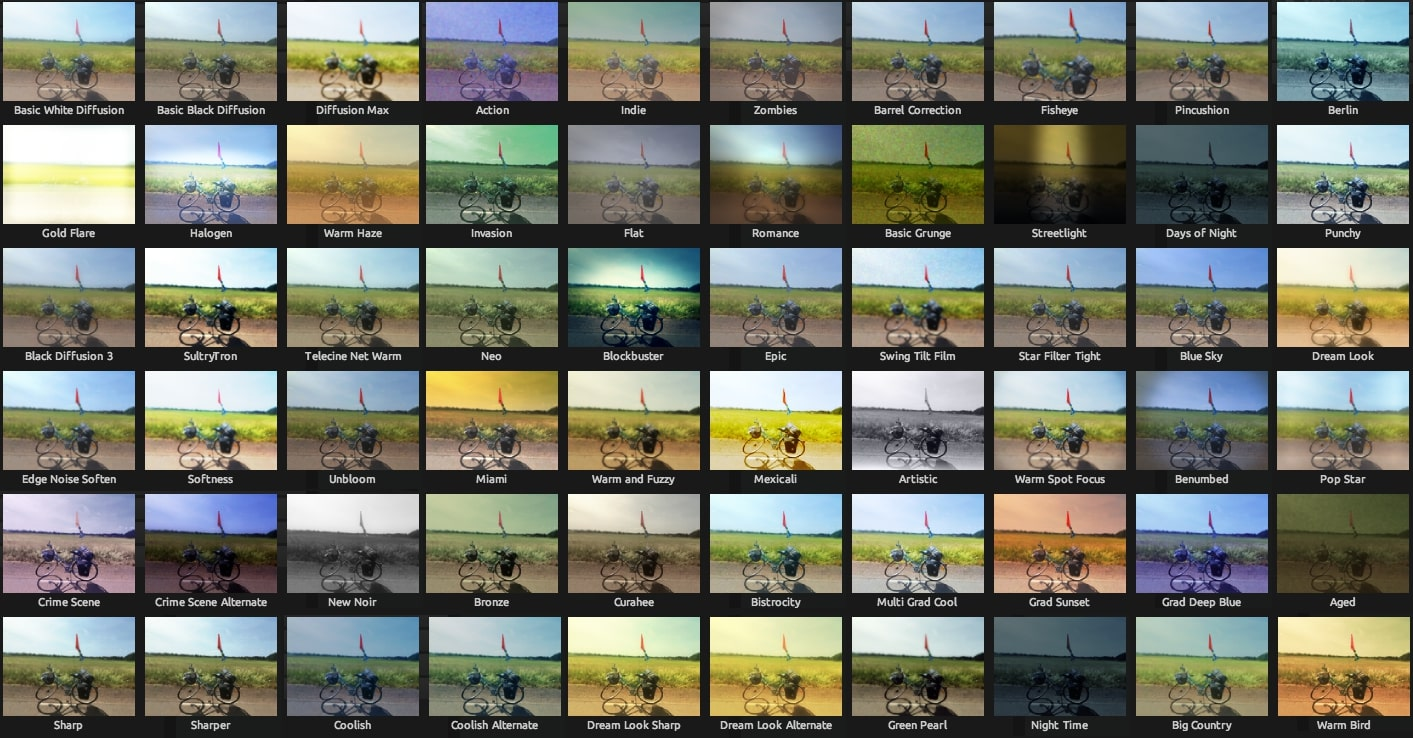
\includegraphics[width=0.99\textwidth]{app.jpg}
	
	\caption[Presets in Adobe Premiere Pro (\textit{Magic Bullet Looks}).]{Preset overview in Adobe Premiere Pro with the plug-in \textit{Magic Bullet Looks}~\cite{premierepro, magicbullet}.}
	\label{figure:app}
	
\end{figure}

Implementing options for the application of those presets is an interesting opportunity for future work. To implement this, different MLT filters can be used or combined. Different options for those MLT filters as video preset filters can be seen in Appendix~\ref{appendix:differentMeltFilter}.













%-------------------------------------------------------------------------------------------------------
\subsubsection*{Advanced Video Processing}

With the implementation of options for advanced video processing tools, other opportunities arise. An online video editing tool with a MLT backend could be implemented. The functionalities could include the cutting of video clips, the application of above described video presets and the manual adjustment of individual video and audio parameters.










%-------------------------------------------------------------------------------------------------------
\subsubsection*{Improvements of the User Interface}


Improvements of the user interface can be implemented to make the adjustment of the RGB colours more intuitive. This could involve a preview of the colour that is being created by adjusting the RGB sliders and that is then applied to the video. An example for this preview can be seen in Figure~\ref{figure:UI}.
To decide which changes in the user interface enhance the usability of the colour adjustment and feel intuitive for the user, extensive testing and user studies could be conducted.

\begin{figure}[H]
	\begin{center}
		\cutpic{0.3cm}{0.65\textwidth}{ApoADC.png}
		\caption[Example for the colour preview of the RGB sliders.]{Example for the preview of the colour, that is being created by adjusting the RGB sliders and then applied to the video.}
		\label{figure:UI}
	\end{center}
\end{figure}



In addition to this, the above described future work opportunities of implementing video presets or an online video editing tool need a design for the user interface as well, to guarantee the usability. 












%-------------------------------------------------------------------------------------------------------
\subsubsection*{Performance Evaluation}


In this thesis project, the results of different methods of applying MLT filters were visually compared. Another interesting aspect is the comparison of the performance of those different methods. For this, the runtime as well as the memory usage could be interesting parameters to observe. 
To ensure accuracy, a separate system or server would be needed, which should be isolated from other processes to prevent interference. Monitoring tools can be used to track the resource usage. 
Those tests can be run on test cases that were developed to represent typical scenarios or more specialised test cases for information with specific restrictions and conditions.
It would be interesting to vary parameters such as the video file size or the amount of applied filters.
This data can then be statistically analysed.












%-------------------------------------------------------------------------------------------------------
\subsubsection*{Audio Filter}

This thesis project focuses on the application of visual filters to a video, especially the adjustment of the RGB values. Aside from this, audio processing plays a role in the processing of videos, too. Similar to the visual content, the audio can enhance the experience and evoke emotions in the viewer. Audio filters can also be used to improve the quality of the recorded audio for example by applying noise suppression or to add context to a scene by adding fitting surrounding noises. In addition to this, simple aspects including the volume or tone can be modified.
The list of filters on the MLT website contains the available audio filters~\cite{melt}.
The implementation of the audio filter integration is an interesting option for future work. To compare different audio filters, the according sound waves of a track could be read out and compared.




In this thesis project, insights on multimedia processing, colour theory and the MLT framework have been gained and contributions have been made to the field. This lead to various options for future work projects.

%The project addressed the complexities of real-time RGB adjustment within the Melt framework and has provided comparisons of various filtering techniques. 






	
	
\end{document}